\section{Magneto-Electric Subbands in Quantum Confined Structures in the presence of Spin-Orbit Interaction}
\label{sec: magneto-electric subbands}

When an electron is confined in a structure of restricted dimensionality(such as quantum well or a quantum wire) and is subjected to a  magnetic field, the electron experiences both electrostatic confinement due to structure and magnetostatic confinement due to the magnetic field. Aa a result, the allowed electronic states are hybrid magneto-electric states which form a subbands. In this chapter, we will derive the dispersion relations in these subbands in the presence of SOC.



\subsection{Spin-Orbit-Interaction in a Solid}
\label{sec: spin orbit interaction in a solid}
According to a well know discussion, we can get nuclear attracted electron's SOC
\begin{align}
	H_{SO}=-\frac{g_ee\hbar}{8m^2c^2}(\pmb{\nabla}V\times\pmb{p})\cdot\pmb{\sigma}=-\frac{e\hbar}{4m^2c^2}(\pmb{\nabla}V\times\pmb{p})\cdot\pmb{\sigma}
	\label{equ: SOC hamiltonian}
\end{align}

Where $\pmb{\sigma}$ is pauli matrices. 

In a solid, a quasi-free electron in the conduction band does not experience the strong nuclear attraction as in an atom. However, it may still see an electric field(or potential gradient) due to internal effects such as the discontinuity of the conduction band in a heterostructure or due to an externally applied E-field. And this field will induce a SOC with the form of Hamiltonian \ref{equ: SOC hamiltonian}. \\

There are two types SOC in Solid which can be classified according to two different inversion asymmetries. First is \tcb{\textit{Structual Inevrsion Asymmetry(SIA)}} and the corresponding \tcb{Rashba Interaction}. Second is \tcb{\textit{Crystallographic Inversion Asymmetry}} and \tcb{Dresselhaus Interaction}. \\

\begin{figure}[H]
	\centering
	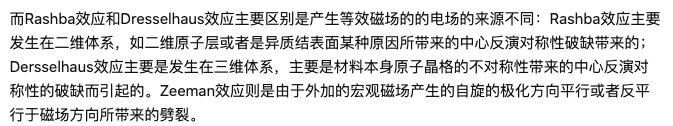
\includegraphics[scale=0.75]{two-soc's-difference}
\end{figure}

\subsubsection{Rashba Interaction}
\label{sec: rashba interaction}
For a crystal electron, we can have 
\begin{align*}
	H^{band}_{SO}=\frac{ge\hbar}{8(m^\star)^2 c^2}\pmb{\nabla}V\cdot(\pmb{\sigma}\times\pmb{p})=-\frac{ge\hbar}{8(m^\star)^2 c^2}\pmb{E}\cdot(\pmb{\sigma}\times\pmb{p})
\end{align*}

Where $m^\star$ is the effective mass. And the Rashba interaction is almost the same form with
\begin{align}
	H_R&=-\pmb{\eta}_R\cdot(\pmb{\sigma}\times\pmb{p})\\
	\pmb{\eta}_R&=-\frac{ge\hbar}{8(m^\star)^2 c^2}\pmb{E}(\pmb{r})
\end{align}

This is the simplistic form, after we consider the band structure effects in a solid, we will get 
\begin{align}
	\pmb{\eta}_R=-\frac{e\hbar}{m^\star(\vec{r})} \frac{\pi \Delta_s(2E_g+\Delta_s)}{E_g(E_g+\Delta_s)(3E_g+2\Delta_s)}\pmb{E}(\vec{r})	
	\label{equ: rashba effect coefeicient}
\end{align}

Where $E_g$ is the band gap of and $\Delta_s$ is the spin-orbit splitting in the valance band.  On the other hand, if there is also magnetic field, we need to re-write our expression with $\pmb{p}+e\pmb{A}$ instead of $\pmb{p}$.
\begin{align*}
	H_R=\pmb{\eta}_R(\vec{r})\cdot [\pmb{\sigma}\times(\pmb{p}+e\pmb{A})]
\end{align*}


\subsubsection{Dresselhaus Interaction}
\label{sec: dresselhaus interaction}
The Pauli Equation \ref{equ: pauli equation} describe a single electrons in a crystal lattice in the absence of any external magnetic field, but in the presence of SOC the equation will become
\begin{align}
	\Big[\frac{\pmb{p}^2}{2m_0}+V_{lattice}-\frac{e\hbar}{4m_0^2c^2}(\pmb{\nabla}V\times\pmb{p})\cdot\pmb{\sigma} \Big][\psi]=E[\psi]
	\label{equ: pauli equation with SOC}	
\end{align}

Where $V_{lattice}$ is the (spatially periodic) electrostatic potential energy due to the ionized atoms in the crystal. And we have the wavefunction should follow Bloch theorem
\begin{align*}
	[\psi]=e^{i \pmb{k}\cdot \pmb{r}}[u_{\pmb{k}}(\vec{r})]=e^{i \pmb{k}\cdot \pmb{r}}\begin{bmatrix}
		u^\uparrow _{\pmb{k}}(\vec{r})\\u^\downarrow _{\pmb{k}}(\vec{r})
	\end{bmatrix}
\end{align*}

Then we can re-write equation \ref{equ: pauli equation with SOC} with substituting the upper Bloch form
\begin{align*}
	\Big[\frac{\pmb{p}^2}{2m_0}+&V_{lattice}-\frac{e\hbar}{4m_0^2c^2}(\pmb{\nabla}V\times\pmb{p})\cdot\pmb{\sigma} \Big][u_{\pmb{k}}(\vec{r})]\\
	&+\hbar\pmb{k}\cdot\Big[\frac{p}{m_0}-\frac{e\hbar}{4m_0^2C^2}(\pmb{\sigma}\times\pmb{\nabla}V) \Big][u_{\pmb{k}}(\vec{r})]=(E_k-\frac{\hbar^2k^2}{2m_0})[u_{\pmb{k}}(\vec{r})]
\end{align*}


The similar equation should be the next expression for $\pmb{k}+\pmb{K}$ with $\pmb{K}$ is the reciprocal lattice vector
\begin{align*}
	\Big[\frac{\pmb{p}^2}{2m_0}+&V_{lattice}-\frac{e\hbar}{4m_0^2c^2}(\pmb{\nabla}V\times\pmb{p})\cdot\pmb{\sigma} \Big][u_{\pmb{k}+\pmb{K}}(\vec{r})]\\
	&+\hbar\pmb{k}\cdot\Big[\frac{p}{m_0}-\frac{e\hbar}{4m_0^2C^2}(\pmb{\sigma}\times\pmb{\nabla}V) \Big][u_{\pmb{k}+\pmb{K}}
	(\vec{r})]\\
	&+\hbar\pmb{K}\cdot\Big[\frac{p}{m_0}-\frac{e\hbar}{4m_0^2C^2}(\pmb{\sigma}\times\pmb{\nabla}V) \Big][u_{\pmb{k}+\pmb{K}}
	(\vec{r})]=(E_k-\frac{\hbar^2(\pmb{k}+\pmb{K})^2}{2m_0})[u_{\pmb{k}+\pmb{K}}(\vec{r})]
\end{align*}
 
 With treating the term $\hbar\pmb{K}\cdot\Big[\frac{p}{m_0}-\frac{e\hbar}{4m_0^2C^2}(\pmb{\sigma}\times\pmb{\nabla}V) \Big]$ as a perturbation ad applying group theoretic results, Dresselhaus derived the SOC Hamiltonian and spin-splitting energies in principal crystallographic directions. And for this direction, it has the form
 \begin{align}
 	H_D=\nu_D \pmb{\sigma}\cdot \pmb{\kappa}
 	\label{equ: dresselhaus type SOC hamiltonian}
 \end{align}
 
 Where 
 \begin{gather*}
 	\kappa_i=\frac{1}{2\hbar^3}\delta_{ijk}[p_i(p_j^2-p_k^2)+(p_j^2-p_k^2)p_i] \footnotemark[1]
 \end{gather*}
 
 \footnotetext[1]{$k_x=\frac{1}{2\hbar^3}[p_x(p_y^2-p_z^2)+(p_y^2-p_z^2)p_x]$} 
 
 
 
 Right now we can see the scheme 
 \begin{figure}[H]
 	\centering	
 	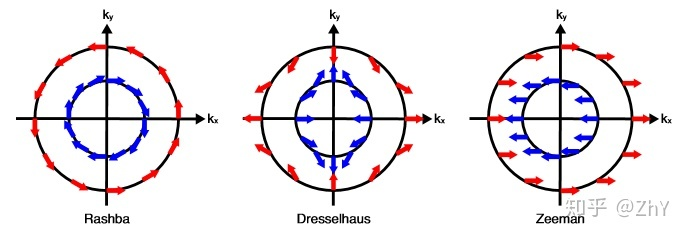
\includegraphics[scale=0.5]{soc}
 	\caption{Two types SOC and Zeeman Effect to show the spin and momentum.}
 	\label{fig: rashba effect and dresselhaus effect's scheme}
 \end{figure}
 
 
 \subsection{Magneto-electric subbands in a 2D electron gas in the presence of spin-orbit interaction}
 \label{sec: 2D subbands}
 
 The general form of Hamiltonian for 2DEG moving in magneto-electric field should be
\begin{align}
	H_{2DEG}=\frac{|\vec{p}+e\vec{A}|^2}{2m^\star}+V(z)+H_Z+H_R+H_D	
	\label{equ: general form hamiltonian of subbands}
\end{align}

Where $H_z$ is Zeeman interaction, $H_R,H_D$ are Rashba and Dresselhaus effect. $V(z)$ comes from the electrostatic potential in $z$ direction. (Typically, this potential comes from the band discontinuity at the hetero-interface or external applied E-field).\\

The key to solve this hamiltonian is to know the fields. Next we will introduce some systems.

\subsubsection{Magnetic field in the plane of the 2DEG}
\label{sec: magnetic field in the plane of 2deg for subbands}

We apply
\begin{gather*}
	\vec{B}=B_x\hat{x}+B_y\hat{y}\\
	\vec{A}=B_yz\hat{x}-B_xz\hat{y}
\end{gather*}

Then we can get 
\begin{align}
	H^{||}_{2DEG}=&\frac{1}{2m^\star}[(p_x+eB_yz)^2+(p_y-eB_xz)^2+p_z^2]+V(z)\\
	\nonumber&-\frac{g}{2}\mu_B[B_x\sigma_x+B_y\sigma_y]-\frac{\eta_R}{\hbar}[(p_x+eB_yz)\sigma_y-(p_y-eB_xz)\sigma_x]\\
	\nonumber&+H_D
	\label{equ: hamiltonian of in plane magnetic field of subbands}
\end{align}

Well, $||$ reminds there is a magnetic field parallel to the plane of 2DEG. here $H_D$ is a little complex cause it has many terms. But we can use one approximation which is $\braket{p_z}^2 >> \braket{p_x}^2, \braket{p_y}^2$. Cause in the material, when we use 2DEG model, the perpendicular direction should be uniform, in the other words, the vertical momentum should be much larger than the transverse ones. With this we can get 
\begin{align*}
	H_D=-\frac{\nu_D}{\hbar^3}p_z^2[(p_x+eB_yz)\sigma_x-(p_y-eB_xz)\sigma_y]
\end{align*}

With Pauli Equation
\begin{align*}
	[H^{||}_{2DEG}][\psi^{||}_{2DEG}(x,y,z)]=E[\psi^{||}_{2DEG}(x,y,z)]
\end{align*}

Where $[H^{||}_{2DEG}]$ is a 2$\times$2 matrix and $[\psi^{||}_{2DEG}(x,y,z)]$ is the 2-component wavefunction. We can easily see $H_{2DEG}^{||}$ is $x,y$ dependent freely, so we can write that
\begin{align*}
	\psi^{||}_{2DEG}=e^{ikx}e^{iky}\lambda(z)
\end{align*}


And then the the Pauli equation taken detailed form becomes
\begin{align}
	\nonumber &\Big\{\frac{\hbar^2k_x^2}{2m^\star}+\frac{\hbar^2k_y^2}{2m^\star}-\frac{\hbar^2}{2m^\star}\frac{\partial^2}{\partial z^2}+V(z)+eB_yz\frac{\hbar k_x}{m^\star}eB_xz\frac{\hbar k_y}{m^\star}+e^2z^2\frac{B_x^2+B_y^2}{2m^\star}\\-
	\nonumber &\frac{g}{2}\mu_B(B_x\sigma_x+B_y\sigma_y)-\frac{\eta_R}{\hbar}[(\hbar k_x+eB_yz)\sigma_y-(\hbar k_y-eB_xz)\sigma_x]\\
	&-\frac{\nu_D}{\hbar^3}p_z^2[(p_x+eB_yz)\sigma_x-(p_y-eB_xz)\sigma_y]\Big\}[\lambda(z)]=E[\lambda(z)]
\end{align}

Where the boundary condition should be 
\begin{align}
  [\lambda(z)](z=d)=[\lambda(z)](z=-d)=[0]
\end{align}

Well here we assume a infinite rectangular potential wall located at $z=d/-d$. If the height of wall is finite, the problem should be much more complicated. On the other hand, we first should set given values of $k_y$ and $E$, then the dispersion relation related on $k_x$ can be obtained, vice versa for $k_y$. Finally, a two variables dependent $E(\pmb{k}_x,\pmb{k}_y)$ can be acquired. \\

But the procedure is not easy because the upper Pauli equation is not a linear equation for $k_x, k_y$ which means it's not an eigen-equation for both $\pmb{k}$. So the first step is to convert this equation to an eigen-equation with the expression
\begin{align}
  [\varsigma(z)]=k_x[\lambda(z)]
\end{align}

Then we get 
\begin{align}
  \{\pmb{B}k_x+\pmb{C}\}[\lambda(z)]=\pmb{A}k_x^2[\lambda(z)]
\end{align}

With 
\begin{empheq}[innerbox={\colorbox[rgb]{0.8,0.8,1.}}]{gather*}
	\pmb{A}=-\frac{\hbar^2}{2m^\star}\pmb{I}\\
	\pmb{B}=eB_yz\frac{\hbar}{m^\star}\pmb{I}-\eta_R[\sigma_y]-\nu[\sigma_x] \\
	\pmb{C}=\frac{\hbar^2k_y^2}{2m^\star}\pmb{I}-\frac{\hbar^2}{2m^\star}\frac{\partial^2}{\partial z^2}\pmb{I}-eB_xz\frac{\hbar k_y}{m^\star}\pmb{I}+V(z)\pmb{I}+\underbrace{......}_{\text{complex}} 
\end{empheq}
	

 Then we can get an eigen-equation of $k_x$
 \begin{align}
  \begin{bmatrix}
  		\pmb{0}&\pmb{I}\\
  		\pmb{A}^{-1}\pmb{C}&\pmb{A}^{-1}B
  \end{bmatrix} \begin{bmatrix}
  	\lambda(z)\\ \varsigma(z)
  \end{bmatrix}=k_x 
  \begin{bmatrix}
  	\lambda(z)\\ \varsigma(z)
  \end{bmatrix}
\end{align}

The following procedure is to find an analytical result of the eigen-equation. This should use some approximations\\

\tcb{First we assume that
\begin{align}
  [\lambda(z)]=\begin{bmatrix}
  	\lambda_1(z)\\ \lambda_2(z)
  \end{bmatrix}=\lambda_0(z)\begin{bmatrix}
  	\alpha \\ \beta
  \end{bmatrix}
\end{align}
\vspace{0.1pt}
\indent $\lambda_0(z)$is space part while $\alpha,\beta$ are spin parts. This is called "variable separartion" because we assume the spin is not denpendent on space. Then we have
\begin{align}
  [\psi^{||}_{2DEG}]=e^{ik_xx}e^{ik_yy}\lambda_0(z)\begin{bmatrix}
  	\alpha \\ \beta
  \end{bmatrix}
\end{align}
\indent And we can define $\braket{z}$ and without generality, we can let it equal to 0 as following.
\begin{align}
  \braket{z}=\int_0^{\infty}\lambda_0(z)z\lambda_0(z)dz=z_0
\end{align}
\indent While the second assumation is that we make the width of the 2DEG is so narrow that the subbands are well separated in enrgy. As a result, we can ignore subband mixing(\textcolor{red}{Why?}). With these two approximations, we can get 
\begin{align}
  \nonumber E_n&\approx \braket{H^{||}_{2DEG}}=\braket{\psi^{||}_{2DEG}|H_{2DEG}|\psi^{||}_{2DEG}}\\
  &=\epsilon_n+\frac{\hbar^2(k_x^2+k_y^2)}{2m^\star}-\frac{g}{2}\mu_B[B_x\sigma_x+B_y\sigma_y]-\eta_R[k_x\sigma_y-k_y\sigma_x]-\underbrace{\nu[k_x\sigma_x-k_y\sigma_y]}_{\nu=\nu_D\braket{\partial^2/ \partial z^2}}
\end{align}
\begin{align}
  [-\frac{\hbar^2}{2m^\star}\frac{\partial^2}{\partial z^2}+\frac{e^2z^2(B_x^2+B_z^2)}{2m^\star}]\lambda_0^n{z}=\epsilon_n \lambda_0^n(z)
\end{align}
\indent With Pauli matrices, we can get 
\begin{align}
 \nonumber E_n [\pmb{I}]&=\overbrace{(\epsilon_n+\frac{\hbar^2(k_x^2+k_y^2)}{2m^\star})}^{\overline{E_n}}[\pmb{I}]-\frac{g}{2}\mu_B\begin{bmatrix}
  	B_y&B_x\\ B_x& -B_y
  \end{bmatrix}-\eta_R \begin{bmatrix}
  	k_x &0 \\ 0& -k_x
  \end{bmatrix}+......\\
  &=\begin{bmatrix}
  	\overline{E_n}-(g/2)\mu_B B_y-\eta_R k_x+\nu k_y & -(g/2)\mu_B B_x +\eta_R k_y -\nu k_x \\
  	-(g/2)\mu_B B_x +\eta_R k_y -\nu k_x & \overline{E_n}+(g/2)\mu_B B_y+\eta_R k_x-\nu k_y ,p
  \end{bmatrix}
\end{align}
\indent After diagonalization of the upper expression, we can get 
\begin{align}
  \boxed{E^{||}_{\pm}=\overline{E_n}\pm \sqrt{(\frac{g}{2}\mu_B B_y+\eta_R k_x-\nu k_y )^2+(\frac{g}{2}\mu_B B_x-\eta_R k_y+\nu k_x )^2}}
\end{align}
\indent And the corresponding eigen-states are 
\begin{empheq}[box=\fbox]{gather*}
	\psi^{||}_{+}(B_x,B_y,k_x,k_y)=\begin{bmatrix}
		-\sin(\theta_k)\\ \cos(\theta_k)
	\end{bmatrix}\\
	\psi_-^{||}=\begin{bmatrix}
		\cos(\theta_k)\\ \sin(\theta_k)
	\end{bmatrix}\\
	\theta_k=\frac{1}{2}\arctan \Big[\frac{(g/2)\mu_B B_y-\eta_R k_y +\nu k_x}{(g/2)\mu_B B_y+\eta_R k_y -\nu k_x} \Big]
\end{empheq}
}







 
 